
In this chapter, we present the design concept of FDPS: the purpose of its development, the basic concept, and the behavior of codes developed using FDPS.

%%%%%%%%%%%%%%%%%%%%%%%%%%%%%%%%%%%%%%%%%%%%%%%%%%%%%%%%%%%%%%%% 
\section{The mission of FDPS}

In the fields of science and engineering, particle method is used for a wide variety of simulations, such as gravitational $N$-body simulation, Smoothed Particle Hydrodynamics (SPH) simulation, vortex method, Moving Particle Semi-implicit (MPS) method, molecular dynamics simulation, and so on. We need high-performance particle simulation codes in order to follow physical phenomena with high spatial resolution, and for long timescales.

We cannot avoid parallelization in order to develop high performance particle simulation codes. For the parallelization, we need to implement the following procedures: dynamic domain decomposition for load balancing, exchange of particles between computing nodes, optimization of communication among nodes, effective use of cache memories and SIMD operation units, and support for accelerators. So far, individual research groups were trying to implement these procedures.

However, the above procedures are necessary for any particle simulation codes. The purpose of the development of FDPS is to provide numerical libraries for implementing these procedures, and reduce researchers' and programmers' burdens. We will be happy if researchers and programmers can use their time more creatively by using FDPS.

%%%%%%%%%%%%%%%%%%%%%%%%%%%%%%%%%%%%%%%%%%%%%%%%%%%%%%%%%%%%%%%%
\section{Basic concept}
In this section, we describe the basic concept of FDPS.

%%%%%%%%%%%%%%%%%%%%%%%%%%%%%%%%
\subsection{Procedures of massively parallel particle simulations}
\label{subsec:pcr_of_massively_parallel_ptcl_sim}

First, we describe our model of massively parallel particle simulations on FDPS. In particle simulations, the set of ordinary differential equations,
\begin{align}
    \frac{d\bm{u}_i}{dt} = \sum_j f(\bm{u}_i,\bm{u}_j) + \sum_s
    g(\bm{u}_i,\bm{v}_s), \label{eq:GoverningEquation}
\end{align}
is numerically integrated, where $\bm{u}_i$ is the quantity vector of $i$-particle. This vector includes quantities of particle $i$, such as mass, position, and velocity. The function $f$ specifies a force exerted by particle $j$ on particle $i$. Hereafter, a particle receiving a force is called $i$-particle, and a particle exerting a force is called $j$-particle. The vector $\bm{v}_s$ is the quantity vector of a superparticle which represents a group of particles that are distant from $i$-particle. The function $g$ specifies a force exerted by a superparticle on a particle. The second term in the left hand side of eq.~(\ref{eq:GoverningEquation}) is a non-zero quantity in the case of long-range forces (e.g. gravity and Coulomb force), while it is zero in the case of short-range forces (e.g. pressure of fluid).

Massively parallel simulation codes integrate the above eq.~(\ref{eq:GoverningEquation}) by taking the following steps (initialization and data I/O are omitted).
\begin{enumerate}
\item In the following two steps, we determine which MPI process handles which particles. \label{item:LoadBalance}
\begin{enumerate}
\item Decompose the whole domain into subdomains, and determine which MPI process handles which subdomains, in order to balance the calculation cost (domain decomposition).
\item MPI processes exchange their particles in order for each MPI process to have particles in its subdomain.
\end{enumerate}

\item Each MPI process gathers quantity vectors of $j$-particles ($\bm{u}_j$) and superparticles ($\bm{v}_s$) required to calculate forces exerted on $i$-th $i$-particle (making interaction lists). \label{item:MakeInteractionList}

\item Each MPI process calculates the right hand of eq.~(\ref{eq:GoverningEquation}) for all of its $i$-particle and obtains $d\bm{u}_i/dt$. \label{item:CalcInteraction}

\item Each MPI process performs the time integration of its $i$-particles by using the quantity vectors of $\bm{u}_i$ and their derivatives $d\bm{u}_i/dt$. \label{item:IntegrateTime}

\item Return to step~\ref{item:LoadBalance}.
\end{enumerate}

%%%%%%%%%%%%%%%%%%%%%%%%%%%%%%%%
\subsection{Division of tasks between users and FDPS}
FDPS handles tasks related to interaction calculation and efficient parallelization and the user-written code performs the rest. The actual function for interaction calculation is supplied by users. Thus, FDPS deals with domain decomposition and exchange of particles (step~\ref{item:LoadBalance}), and making interaction lists. On the other hand, the user code is responsible for actual calculation of forces (step~\ref{item:CalcInteraction}), and time integration (step~\ref{item:IntegrateTime}). Users can avoid the development of complicated codes necessary for realizing massively parallel program, by utilizing FDPS APIs.

%%%%%%%%%%%%%%%%%%%%%%%%%%%%%%%%
\subsection{Users' tasks}
\label{subsec:things_to_do_by_users}

Users's tasks are as follows.
\begin{itemize}
\item Define a particle (Chap.~\ref{chap:user_defined}). Users need to specify quantities of particles, \textit{i.e.} the quantity vector $\bm{u}_i$ in eq.~(\ref{eq:GoverningEquation}), which contains quantities such as position, velocity, acceleration, chemical composition, and particle size.

\item Define interaction (Chap.~\ref{chap:user_defined}). Users need to specify the interaction between particles, \textit{i.e.} the function $f$ and $g$ in eq.~(\ref{eq:GoverningEquation}), such as gravity, Coulomb force, and pressure.

\item Call FDPS APIs (Chap.~\ref{chap:API_spec_list}).

\item Time integration of particles, diagnostic, output etc.

\end{itemize}

%%%%%%%%%%%%%%%%%%%%%%%%%%%%%%%%
\subsection{Complement}
The right hand side of eq.~(\ref{eq:GoverningEquation}), the particle-particle interactions, is strictly of two-body nature. FDPS APIs can not be used to implement three-particle interactions. However, for example, FDPS has APIs to return neighbor lists. Users can calculate three- or more-body interactions, using these neighbor lists.

Calculation steps in section~\ref{subsec:pcr_of_massively_parallel_ptcl_sim} imply that all particles have one same timestep. FDPS APIs do not support individual timestep scheme. However, users can develop a particle simulation code with individual timestep scheme, using the Particle-Particle Particle Tree method.

%%%%%%%%%%%%%%%%%%%%%%%%%%%%%%%%%%%%%%%%%%%%%%%%%%%%%%%%%%%%%%%%
\section{The structure of a simulation code with FDPS}
\label{sec:overview_action}
In this section, we first overview the structure of a simple simulation code written using FDPS, not FDPS Fortran/C interface. Then, we describe the structure of a code written using FDPS Fortran/C interface.

%%%%%%%%%%%%%%%%%%%%%%%%%%%%%%%%
\subsection{FDPS}
In a code with FDPS, three FDPS-supplied classes and several user-defined classes are used.
\begin{itemize}

\item DomainInfo class. This class contains the information of all the subdomains, and APIs for domain decomposition.

\item ParticleSystem class. This class contains the information of all particles in each MPI process, and APIs for the exchange of
  particles among MPI processes.

\item TreeForForce class. This class contains tree structure made from particle distribution, and APIs for making interaction lists.

\item User-defined classes. These classes include the definitions of particles and interactions.
\end{itemize}

These classes communicate with each other. This is illustrated in Fig.~\ref{fig:brief_interface}. The communication in this figure corresponds to steps 1 and 2, and to initialization (step~0).
\begin{enumerate}
\item[0.] Users give a user-defined particle class to ParticleSystem class, and a function object to TreeForForce class. These are not class inheritance. The particle class is used as a template argument of ParticleSystem class, and the function object is used as an argument of APIs in TreeForForce class.

\item[1.] Do load balancing in the following two steps.
\begin{enumerate}
\item The user code calls APIs for domain decomposition in DomainInfo class. Particle information is transferred from ParticleSystem class to DomainInfo class (red text and arrows).
\item The user code calls APIs for exchange of particles in ParticleSystem class. Information of subdomains is transferred from DomainInfo class to ParticleSystem class (blue text and arrows).
\end{enumerate}

\item[2.] Do the force calculation in the following steps.
\begin{enumerate}
\item[(a)] The user code calls force calculation API.

\item[(b)] FDPS makes interaction lists in TreeForForce
  class. Information of subdomains and particles is transferred from
  DomainInfo and ParticleSystem classes (green text and arrows).
\end{enumerate}

\item[3.] FDPS calls an user-defined function object. This API is included in TreeForForce class. Interactions are calculated, and the results are transferred from TreeForForce class to ParticleSystem class (gray text and arrows).
\end{enumerate}

%%%%%%%%%%%%%%%%%%%%%%%%%%%%%%%%
\subsection{FDPS Fortran/C interface}
All the APIs described in the previous section are implemented in FDPS Fortran/C interface. Therefore, the structure of Fortran/C code is similar to that of C++ code. The complete list of the APIs in FDPS Fortran/C interface is given in Chap.~\ref{chap:API_spec_list}.

% Figure
\begin{figure}[h]
\centering
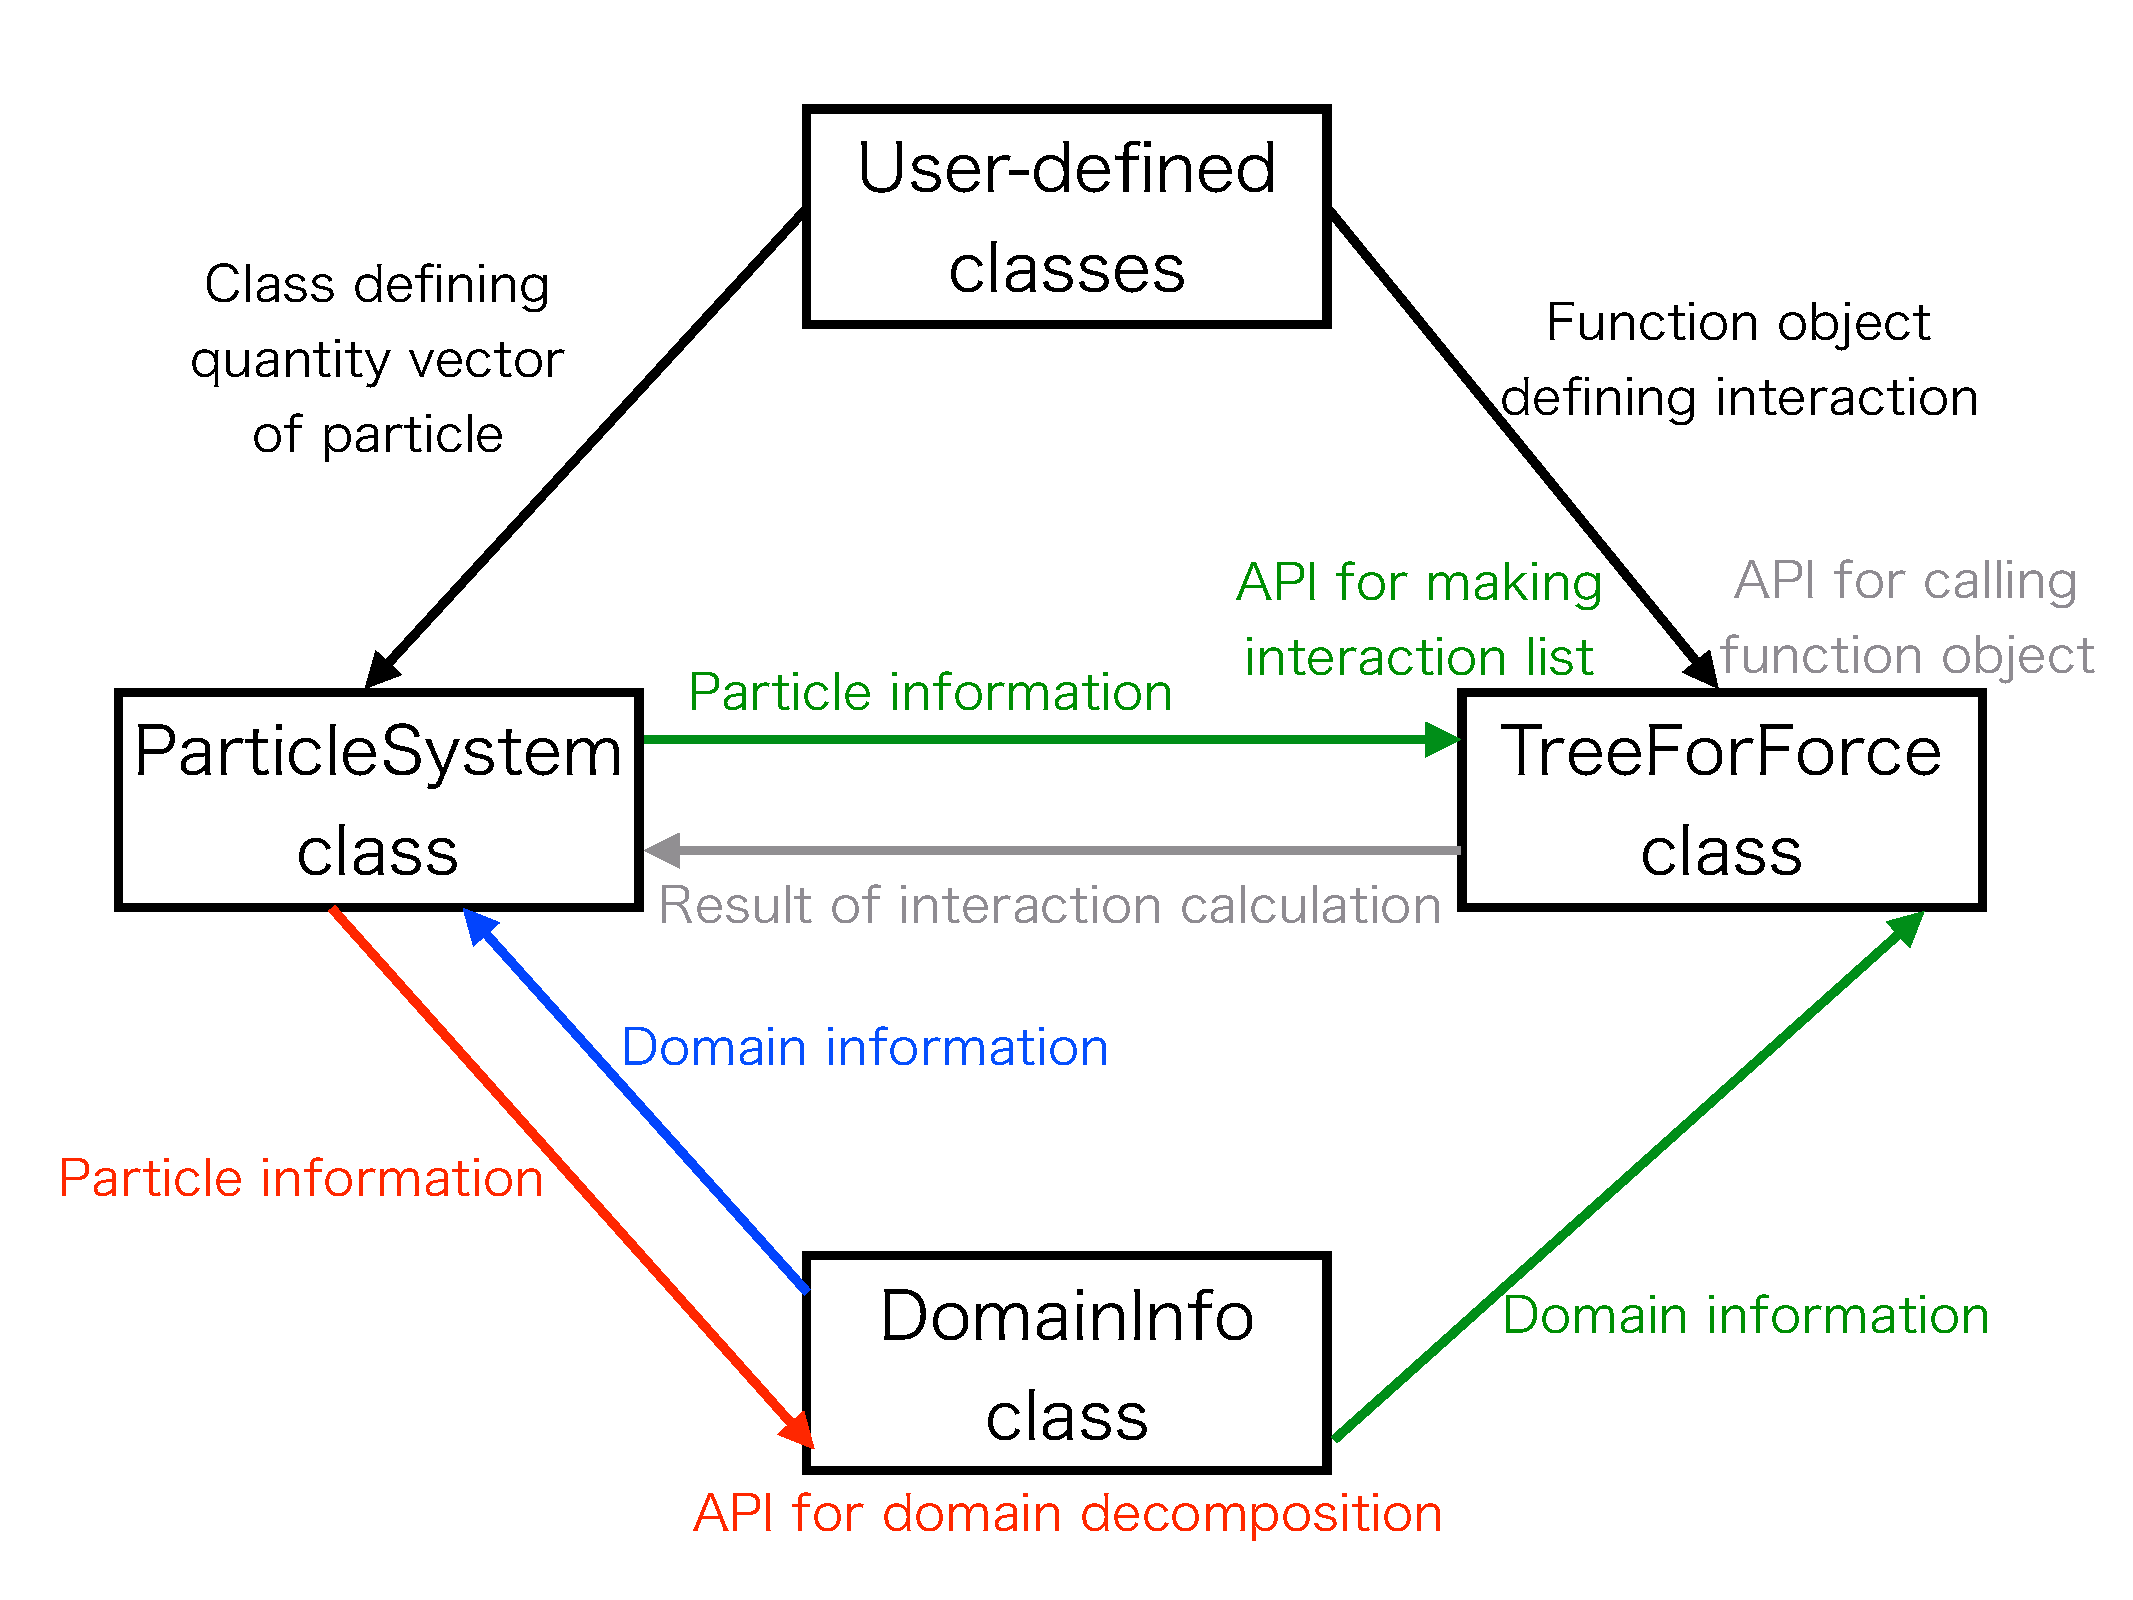
\includegraphics[width=0.75\textwidth]{./fig/illustration.pdf}
\caption{Illustration of module interface and data transfer.}
\label{fig:brief_interface}
\end{figure}
